%---------------------------------------------------------------------------
\begin{frame}[t]
\frametitle{TCF {\small Turbulent Channel Flow at $ Re_\tau=395 $}}
\textbf{LES for wall bounded flows?}
\vfill
\onslide<1->{
\textbf{Problem:} 
\begin{itemize}
\item LES models cannot accurately simulate boundary layers without stretched meshes
\end{itemize}}
\onslide<2->{
\textbf{Solution:}
\begin{itemize}
\item Use of weak boundary conditions (Nitche's method)
\item Impose the tangential traction on the wall from a wall law model [Bazilevs \textit{et al} '07]
\item We aslo impose weakly the wall-normal component
\end{itemize}
} 
\vfill
\end{frame}
%---------------------------------------------------------------------------
\begin{frame}[t]
\frametitle{TCF {\small Turbulent Channel Flow at $ Re_\tau=395 $}}
\textbf{Weak boundary conditions:}
 \vspace*{-0.3cm}
  \begin{figure}
    \centering	
    \only<1-3>{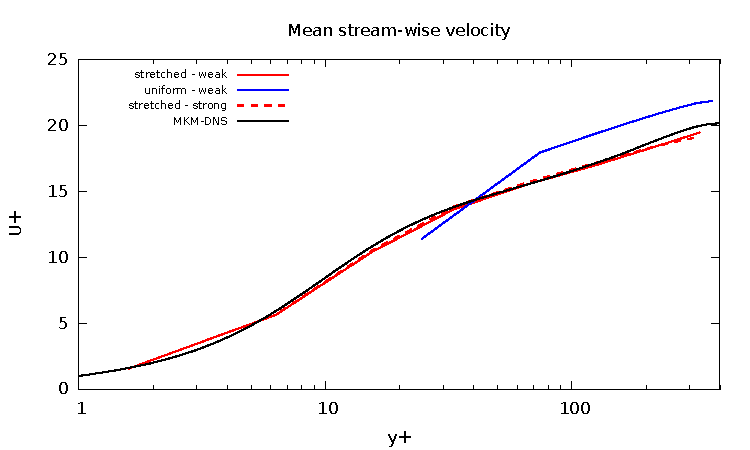
\includegraphics[width=0.75\textwidth]{Figures/SVMS_TCF/umean}}
    \only<4>{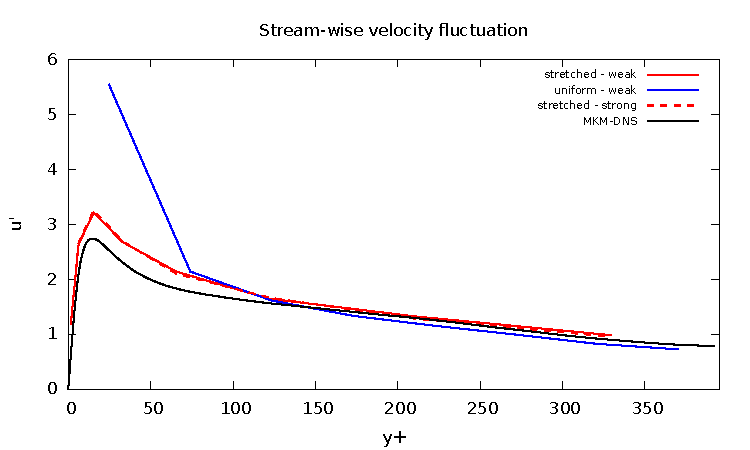
\includegraphics[width=0.75\textwidth]{Figures/SVMS_TCF/ufluc}}
  \end{figure}
  \vspace*{-0.5cm}
   \begin{overlayarea}{\textwidth}{1.5cm}
 \only<2->{
 \begin{itemize}
  	\item \alert<2>{We recover the strong BC results} when stretched mesh is used.
  	\only<3->{\item \alert<3>{Acceptable results} for uniform meshes.}
  \end{itemize}}
  \end{overlayarea}
\end{frame}